\documentclass[11pt,a4paper]{report}
\usepackage[textwidth=37em,vmargin=30mm]{geometry}
\usepackage{calc,xunicode,amsmath,amssymb,paralist,enumitem,tabu,booktabs,datetime2,xeCJK,xeCJKfntef,listings}
\usepackage{tocloft,fancyhdr,tcolorbox,xcolor,graphicx,eso-pic,xltxtra,xelatexemoji}

\newcommand{\envyear}[0]{2025}
\newcommand{\envdatestr}[0]{2025-01-30}
\newcommand{\envfinaldir}[0]{webdb/2025/20250130/final}

\usepackage[hidelinks]{hyperref}
\hypersetup{
    colorlinks=false,
    pdfpagemode=FullScreen,
    pdftitle={Web Digest - \envdatestr}
}

\setlength{\cftbeforechapskip}{10pt}
\renewcommand{\cftchapfont}{\rmfamily\bfseries\large\raggedright}
\setlength{\cftbeforesecskip}{2pt}
\renewcommand{\cftsecfont}{\sffamily\small\raggedright}

\setdefaultleftmargin{2em}{2em}{1em}{1em}{1em}{1em}

\usepackage{xeCJK,xeCJKfntef}
\xeCJKsetup{PunctStyle=plain,RubberPunctSkip=false,CJKglue=\strut\hskip 0pt plus 0.1em minus 0.05em,CJKecglue=\strut\hskip 0.22em plus 0.2em}
\XeTeXlinebreaklocale "zh"
\XeTeXlinebreakskip = 0pt


\setmainfont{Brygada 1918}
\setromanfont{Brygada 1918}
\setsansfont{IBM Plex Sans}
\setmonofont{JetBrains Mono NL}
\setCJKmainfont{Noto Serif CJK SC}
\setCJKromanfont{Noto Serif CJK SC}
\setCJKsansfont{Noto Sans CJK SC}
\setCJKmonofont{Noto Sans CJK SC}

\setlength{\parindent}{0pt}
\setlength{\parskip}{8pt}
\linespread{1.15}

\lstset{
	basicstyle=\ttfamily\footnotesize,
	numbersep=5pt,
	backgroundcolor=\color{black!5},
	showspaces=false,
	showstringspaces=false,
	showtabs=false,
	tabsize=2,
	captionpos=b,
	breaklines=true,
	breakatwhitespace=true,
	breakautoindent=true,
	linewidth=\textwidth
}






\newcommand{\coverpic}[2]{
    % argv: itemurl, authorname
    Cover photo by #2~~(\href{#1}{#1})
}
\newcommand{\makeheader}[0]{
    \begin{titlepage}
        % \newgeometry{hmargin=15mm,tmargin=21mm,bmargin=12mm}
        \begin{center}
            
            \rmfamily\scshape
            \fontspec{BaskervilleF}
            \fontspec{Old Standard}
            \fontsize{59pt}{70pt}\selectfont
            WEB\hfill DIGEST
            
            \vfill
            % \vskip 30pt
            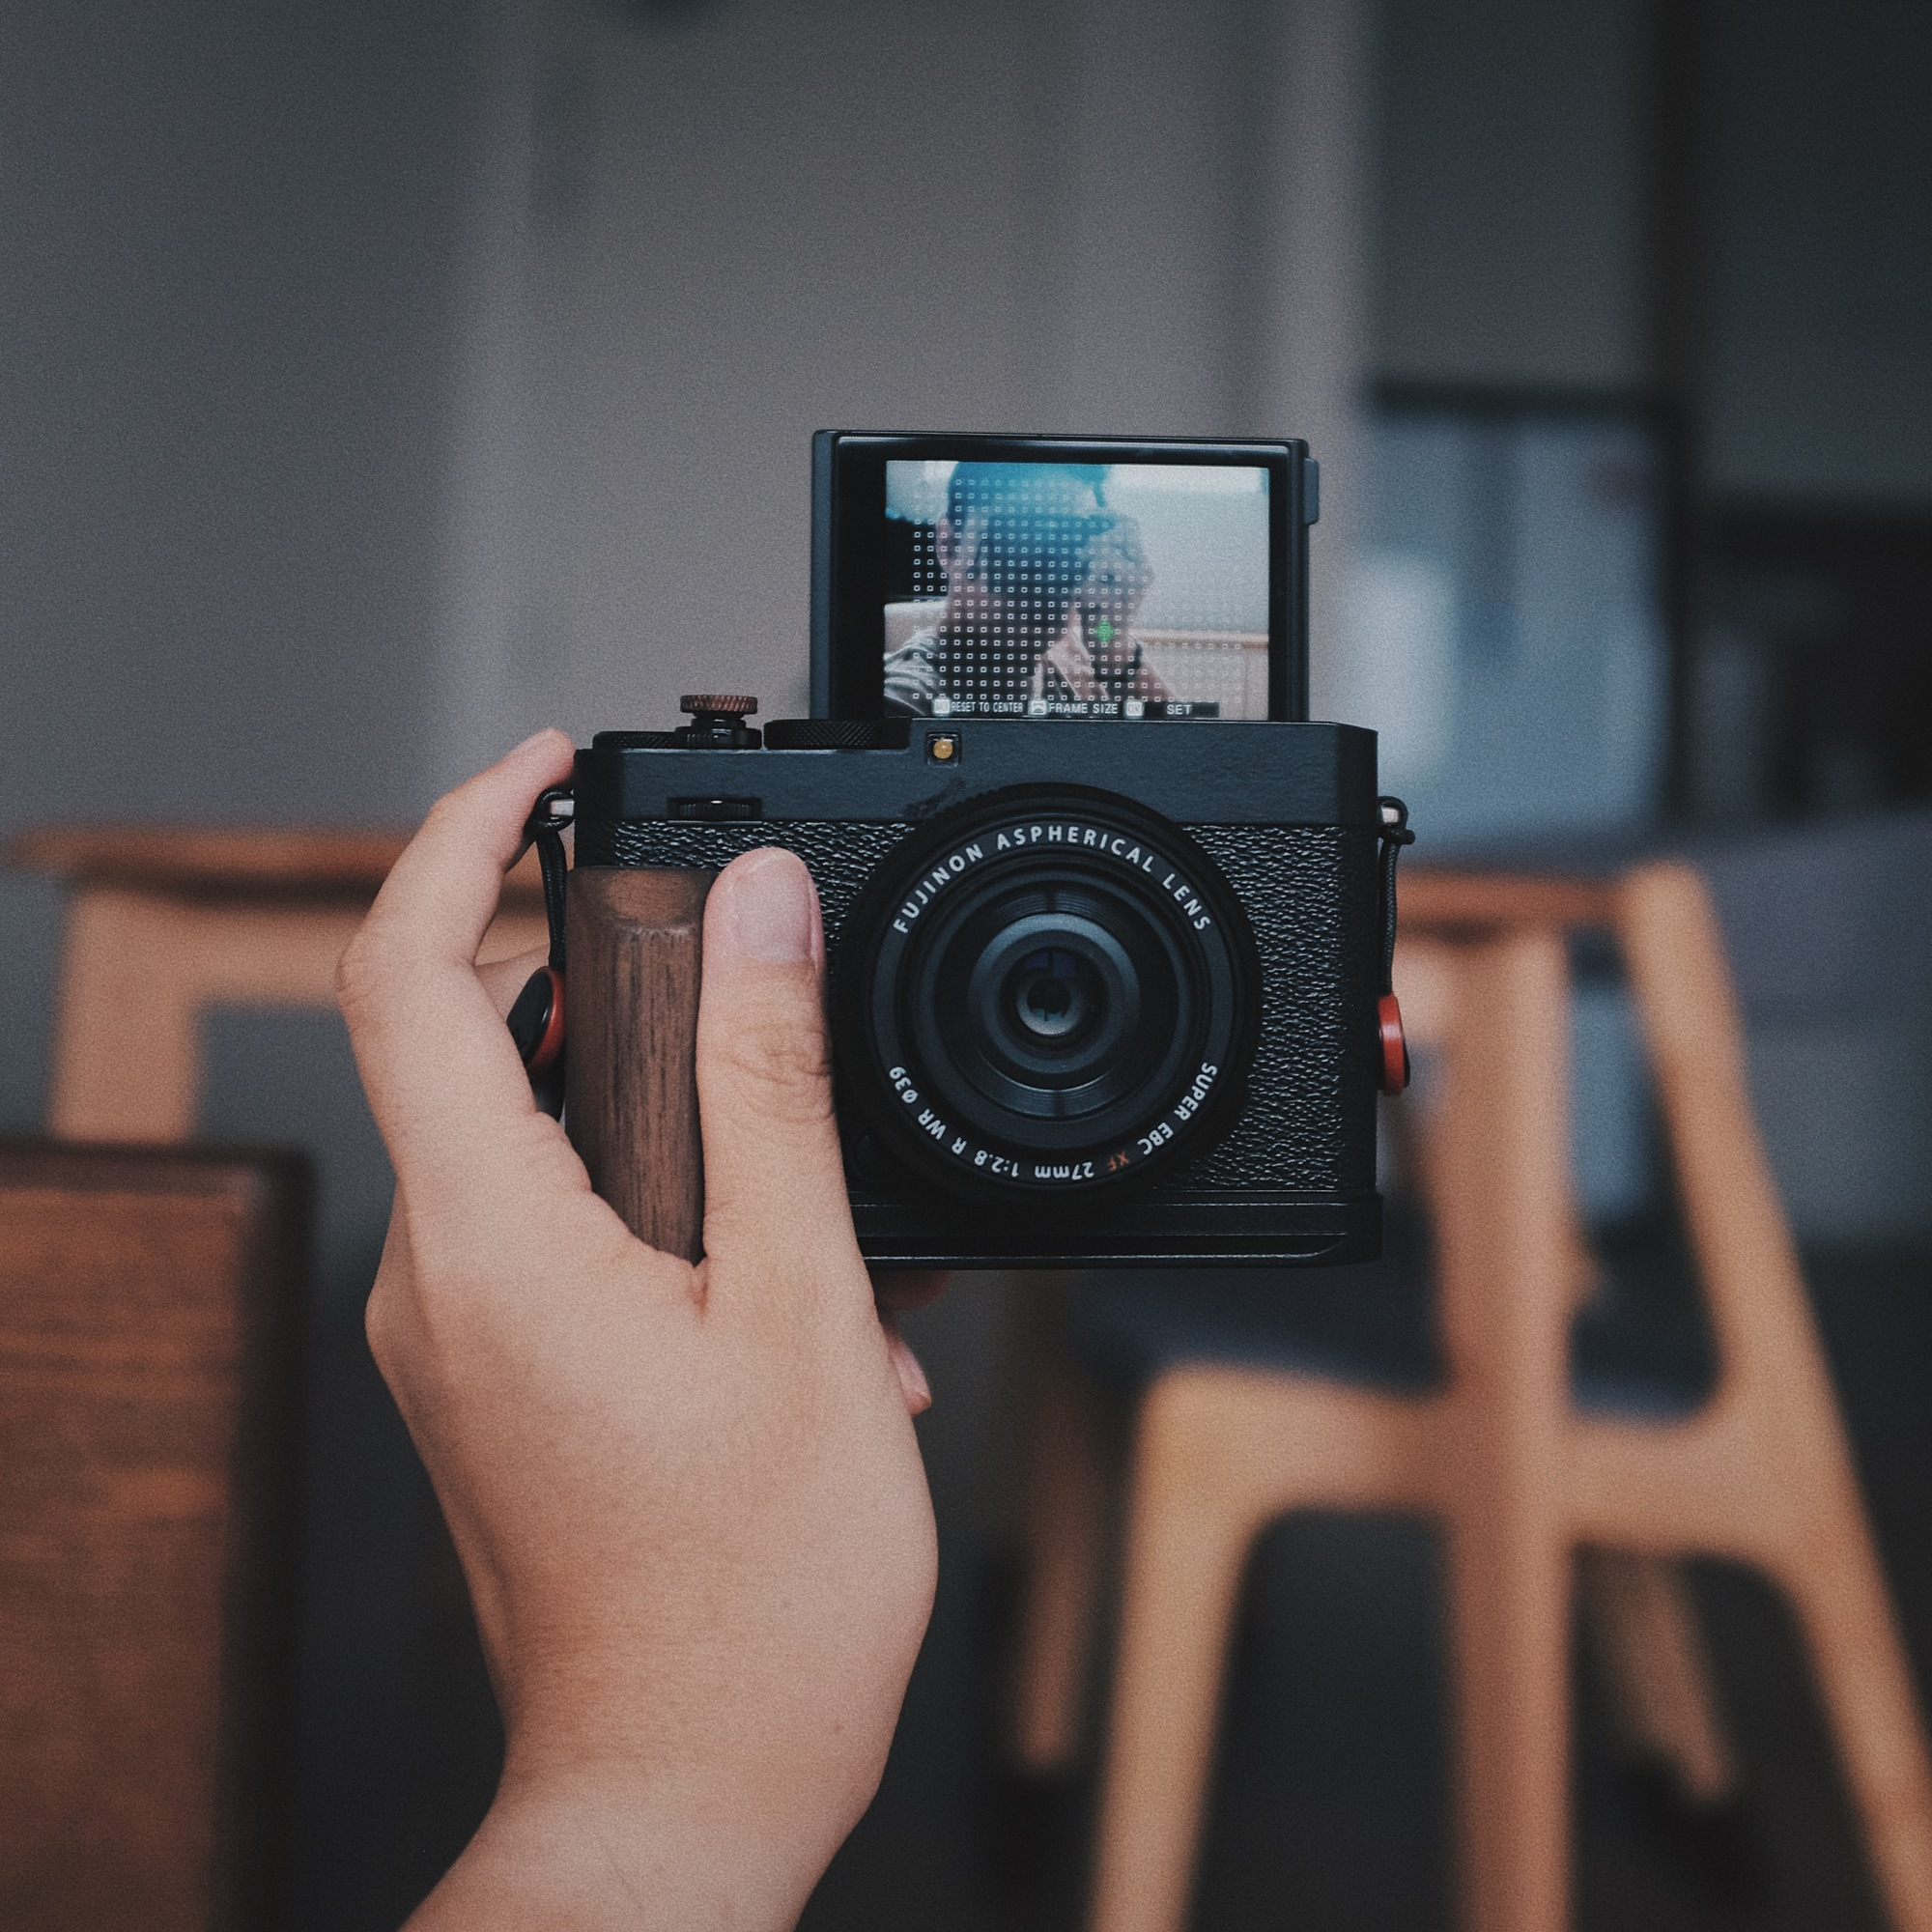
\includegraphics[width=\linewidth]{\envfinaldir/coverpic-prod.jpg}\par
            % \vskip 30pt
            \vfill

            \normalsize\rmfamily\scshape
            \copyright{} The Web Digest Project \hfill\large \envdatestr
        \end{center}
    \end{titlepage}
    % \restoregeometry
}
\newcommand{\simplehref}[1]{%
    \textcolor{blue!80!green}{\href{#1}{#1}}%
}
\renewcommand{\contentsname}{\center\Huge\sffamily\bfseries Contents\par\vskip 20pt}
\newcounter{ipartcounter}
\setcounter{ipartcounter}{0}
\newcommand{\ipart}[1]{
    % \vskip 20pt
    \clearpage
    \stepcounter{ipartcounter}
    \phantomsection
    \addcontentsline{toc}{chapter}{#1}
    % \begin{center}
    %     \Huge
    %     \sffamily\bfseries
    %     #1
    % \end{center}
    % \vskip 20pt plus 7pt
}
\newcounter{ichaptercounter}
\setcounter{ichaptercounter}{0}
\newcommand{\ichapter}[1]{
    % \vskip 20pt
    \clearpage
    \stepcounter{ichaptercounter}
    \phantomsection
    \addcontentsline{toc}{section}{\numberline{\arabic{ichaptercounter}}#1}
    \begin{center}
        \Huge
        \sffamily\bfseries
        #1
    \end{center}
    \vskip 20pt plus 7pt
}
\newcommand{\entrytitlefont}[1]{\subsection*{\raggedright\Large\sffamily\bfseries#1}}
\newcommand{\entryitemGeneric}[2]{
    % argv: title, url
    \parbox{\linewidth}{
        \entrytitlefont{#1}\par\vskip 5pt
        \footnotesize\ttfamily\mdseries
        \simplehref{#2}
    }\vskip 11pt plus 11pt minus 1pt
}
\newcommand{\entryitemGithub}[3]{
    % argv: title, url, desc
    \parbox{\linewidth}{
        \entrytitlefont{#1}\par\vskip 5pt
        \footnotesize\ttfamily\mdseries
        \simplehref{#2}\par\vskip 5pt
        \small\rmfamily\mdseries#3
    }\vskip 11pt plus 11pt minus 1pt
}
\newcommand{\entryitemAp}[3]{
    % argv: title, url, desc
    \parbox{\linewidth}{
        \entrytitlefont{#1}\par\vskip 5pt
        \footnotesize\ttfamily\mdseries
        \simplehref{#2}\par\vskip 5pt
        \small\rmfamily\mdseries#3
    }\vskip 11pt plus 11pt minus 1pt
}
\newcommand{\entryitemHackernews}[3]{
    % argv: title, hnurl, rawurl
    % \parbox{\linewidth}{
    %     \entrytitlefont{#1}\par\vskip 5pt
    %     \footnotesize\ttfamily\mdseries
    %     \simplehref{#3}\par
    %     \textcolor{black!50}{\href{#2}{#2}}
    % }\vskip 11pt plus 11pt minus 1pt
    \begin{minipage}{\linewidth}
            \entrytitlefont{#1}\par\vskip 5pt
            \footnotesize\ttfamily\mdseries
            \simplehref{#3}\par
            \textcolor{black!50}{\href{#2}{#2}}
    \end{minipage}\par\vskip 11pt plus 11pt minus 1pt
}







\begin{document}

\makeheader

\tableofcontents\clearpage




\ipart{Developers}
\ichapter{Hacker News}
\entryitemTwoLinks{Exposed DeepSeek database leaking sensitive information, including chat history}{https://news.ycombinator.com/item?id=42871371}{https://www.wiz.io/blog/wiz-research-uncovers-exposed-deepseek-database-leak}

\entryitemTwoLinks{Making the video that made Gorillaz}{https://news.ycombinator.com/item?id=42870990}{https://animationobsessive.substack.com/p/making-the-video-that-made-gorillaz}

\entryitemTwoLinks{Dead Games}{https://news.ycombinator.com/item?id=42870230}{https://garry.net/posts/dead-games}

\entryitemTwoLinks{Waymo to test its autonomous driving technology in over 10 new cities}{https://news.ycombinator.com/item?id=42870056}{https://www.reuters.com/business/autos-transportation/alphabets-waymo-test-its-autonomous-driving-technology-over-10-new-cities-2025-01-29/}

\entryitemTwoLinks{SmolGPT: A minimal PyTorch implementation for training a small LLM from scratch}{https://news.ycombinator.com/item?id=42868770}{https://github.com/Om-Alve/smolGPT}

\entryitemTwoLinks{Adding iodine to salt played a role in cognitive improvements: research (2013)}{https://news.ycombinator.com/item?id=42868718}{https://www.discovermagazine.com/health/how-adding-iodine-to-salt-boosted-americans-iq}

\entryitemTwoLinks{No Man's Sky's update introduces billions of new stars, planets, and more}{https://news.ycombinator.com/item?id=42868618}{https://blog.playstation.com/2025/01/29/no-mans-skys-latest-update-introduces-billions-of-new-stars-planets-and-more-today/}

\entryitemTwoLinks{"We're building a new static type checker for Python"}{https://news.ycombinator.com/item?id=42868576}{https://twitter.com/charliermarsh/status/1884651482009477368}

\entryitemTwoLinks{Intel doesn't know how to be a foundry, Tim Cook reportedly said in 2011}{https://news.ycombinator.com/item?id=42868531}{https://www.tomshardware.com/tech-industry/tsmc-founder-says-tim-cook-told-him-intel-did-not-know-how-to-be-a-foundry}

\entryitemTwoLinks{An analysis of DeepSeek's R1-Zero and R1}{https://news.ycombinator.com/item?id=42868390}{https://arcprize.org/blog/r1-zero-r1-results-analysis}

\entryitemTwoLinks{On DeepSeek and export controls}{https://news.ycombinator.com/item?id=42866905}{https://darioamodei.com/on-deepseek-and-export-controls}

\entryitemTwoLinks{Why DeepSeek had to be open source}{https://news.ycombinator.com/item?id=42866201}{https://www.getlago.com/blog/deepseek-open-source}

\entryitemTwoLinks{A story about restoring and upgrading a Commodore Amiga 1000}{https://news.ycombinator.com/item?id=42865867}{https://celso.io/posts/2025/01/26/the-first-perfect-computer/}

\entryitemTwoLinks{Google Pixel 4a's old firmware is gone, trapping users on buggy battery update}{https://news.ycombinator.com/item?id=42865619}{https://www.androidcentral.com/phones/google-pixel-4as-old-firmware-is-gone-trapping-users-on-the-buggy-battery-update}

\entryitemTwoLinks{Complete hardware and software setup for running Deepseek-R1 locally}{https://news.ycombinator.com/item?id=42865575}{https://twitter.com/carrigmat/status/1884244369907278106}

\entryitemTwoLinks{OpenAI Furious DeepSeek Might Have Stolen All the Data OpenAI Stole from Us}{https://news.ycombinator.com/item?id=42865527}{https://www.404media.co/openai-furious-deepseek-might-have-stolen-all-the-data-openai-stole-from-us/}

\entryitemTwoLinks{Cali's AG Tells AI Companies Almost Everything They're Doing Might Be Illegal}{https://news.ycombinator.com/item?id=42865174}{https://gizmodo.com/californias-ag-tells-ai-companies-practically-everything-theyre-doing-might-be-illegal-2000555896}

\entryitemTwoLinks{I do not want AI to "polish" me}{https://news.ycombinator.com/item?id=42864854}{https://thebloggess.com/2025/01/28/no-i-do-not-want-ai-to-polish-me/}

\entryitemTwoLinks{Seagate: 'new' hard drives used for tens of thousands of hours}{https://news.ycombinator.com/item?id=42864788}{https://www.tomshardware.com/pc-components/hdds/german-seagate-customers-say-their-new-hard-drives-were-actually-used-resold-hdds-reportedly-used-for-tens-of-thousands-of-hours}

\entryitemTwoLinks{Our phones are killing our ability to feel sexy (2024)}{https://news.ycombinator.com/item?id=42864595}{https://catherineshannon.substack.com/p/your-phone-is-why-you-dont-feel-sexy}\ichapter{Phoronix}
\entryitemGeneric{\hskip 0pt{}Open-Source RADV Radeon Driver Support For RDNA4: "Should Be Good Enough"}{https://www.phoronix.com/news/Mesa-25.0-RADV-RDNA4-State}

\entryitemGeneric{\hskip 0pt{}X.Org / FreeDesktop.org Encounters New Cloud Crisis: Needs New Infrastructure Very Soon}{https://www.phoronix.com/news/2025-XOrg-FreeDesktop-Cloud}

\entryitemGeneric{\hskip 0pt{}PyTorch 2.6 Delivers FP16 Support For x86 CPUs, Better Intel GPU Experience}{https://www.phoronix.com/news/PyTorch-2.6-Released}

\entryitemGeneric{\hskip 0pt{}Ubuntu Developers Moving From IRC To Matrix For Real-Time Communication}{https://www.phoronix.com/news/Ubuntu-Developers-Matrix}

\entryitemGeneric{\hskip 0pt{}NVIDIA GeForce RTX 5080 Linux GPU Compute Performance}{https://www.phoronix.com/review/nvidia-geforce-rtx5080-linux}

\entryitemGeneric{\hskip 0pt{}GNU C Library 2.41 Released With New C23 Features, Intel / AMD / Arm CPU Optimizations}{https://www.phoronix.com/news/GNU-C-Library-glibc-2.41}

\entryitemGeneric{\hskip 0pt{}Bytedance Praises eBPF - Notes 10\% Improvement In Network Throughput}{https://www.phoronix.com/news/Bytedance-eBPF-10p-Networking}

\entryitemGeneric{\hskip 0pt{}Mesa 25.0 Sees New Driver Code To Further Enhance RadeonSI + ACO}{https://www.phoronix.com/news/Mesa-25.0-Better-RadeonSI-ACO}

\entryitemGeneric{\hskip 0pt{}Ubuntu's Snapdragon X1 Elite Laptop Support Enables Experimental Hardware Video Decode}{https://www.phoronix.com/news/Ubuntu-Snapdragon-More-Features}\ichapter{Dribbble}
\entryitemGeneric{\hskip 0pt{}Puzzle Fintech Website Design}{https://dribbble.com/shots/25501121-Puzzle-Fintech-Website-Design}

\entryitemGeneric{\hskip 0pt{}Team Heyo}{https://dribbble.com/shots/25539716-Team-Heyo}

\entryitemGeneric{\hskip 0pt{}DeepSeek logo redesign}{https://dribbble.com/shots/25543483-DeepSeek-logo-redesign}

\entryitemGeneric{\hskip 0pt{}Abstro 8}{https://dribbble.com/shots/25546566-Abstro-8}

\entryitemGeneric{\hskip 0pt{}Top of the World™ Hunt Club}{https://dribbble.com/shots/25545423-Top-of-the-World-Hunt-Club}

\entryitemGeneric{\hskip 0pt{}HappyDev - Logo Design (sold)}{https://dribbble.com/shots/25544140-HappyDev-Logo-Design-sold}

\entryitemGeneric{\hskip 0pt{}Apparel}{https://dribbble.com/shots/25538973-Apparel}

\entryitemGeneric{\hskip 0pt{}B}{https://dribbble.com/shots/25536900-B}

\entryitemGeneric{\hskip 0pt{}2024 Logo Design Recap Pt.1}{https://dribbble.com/shots/25534698-2024-Logo-Design-Recap-Pt-1}

\entryitemGeneric{\hskip 0pt{}De Nieuwe Gemeente - Church Brand}{https://dribbble.com/shots/25537128-De-Nieuwe-Gemeente-Church-Brand}

\entryitemGeneric{\hskip 0pt{}Speed Test App Ui Design}{https://dribbble.com/shots/25535763-Speed-Test-App-Ui-Design}

\entryitemGeneric{\hskip 0pt{}Plexo mobile app}{https://dribbble.com/shots/25534405-Plexo-mobile-app}

\entryitemGeneric{\hskip 0pt{}Vintage Inspired}{https://dribbble.com/shots/25538473-Vintage-Inspired}

\entryitemGeneric{\hskip 0pt{}Illustration set}{https://dribbble.com/shots/25522996-Illustration-set}

\entryitemGeneric{\hskip 0pt{}Dyna - Logo Design}{https://dribbble.com/shots/25525428-Dyna-Logo-Design}

\entryitemGeneric{\hskip 0pt{}B}{https://dribbble.com/shots/25524895-B}

\entryitemGeneric{\hskip 0pt{}Godzilla Logo}{https://dribbble.com/shots/25525727-Godzilla-Logo}

\entryitemGeneric{\hskip 0pt{}Peregrine Engineering®}{https://dribbble.com/shots/25527465-Peregrine-Engineering}

\entryitemGeneric{\hskip 0pt{}VCC Unused Logo Concept - V4}{https://dribbble.com/shots/25525024-VCC-Unused-Logo-Concept-V4}

\entryitemGeneric{\hskip 0pt{}2024 Logo Design Recap Pt.1}{https://dribbble.com/shots/25525396-2024-Logo-Design-Recap-Pt-1}

\entryitemGeneric{\hskip 0pt{}M for Mountain Logo Design (Unused for Sale)}{https://dribbble.com/shots/25524897-M-for-Mountain-Logo-Design-Unused-for-Sale}

\entryitemGeneric{\hskip 0pt{}Tattooed Devil Horns}{https://dribbble.com/shots/25520911-Tattooed-Devil-Horns}

\entryitemGeneric{\hskip 0pt{}Fitness and Step Count app UI Design}{https://dribbble.com/shots/25518949-Fitness-and-Step-Count-app-UI-Design}

\entryitemGeneric{\hskip 0pt{}Plexo}{https://dribbble.com/shots/25519637-Plexo}


\ipart{Developers~~~~(zh-Hans)}
\ichapter{Solidot}
\entryitemGeneric{\hskip 0pt{}研究估计到 2100 年欧洲高温死亡人数增加五成}{https://www.solidot.org/story?sid=80443}

\entryitemGeneric{\hskip 0pt{}Google 开源 Pebble 智能手表操作系统}{https://www.solidot.org/story?sid=80442}

\entryitemGeneric{\hskip 0pt{}用开源方法复现 DeepSeek-R1}{https://www.solidot.org/story?sid=80441}

\entryitemGeneric{\hskip 0pt{}Onlyfans 成功背后的心理学}{https://www.solidot.org/story?sid=80440}

\entryitemGeneric{\hskip 0pt{}科学家通过黑洞合并事件验证宇宙镜像对称性}{https://www.solidot.org/story?sid=80439}

\entryitemGeneric{\hskip 0pt{}研究揭示 PM2.5 毒理学机制}{https://www.solidot.org/story?sid=80438}

\entryitemGeneric{\hskip 0pt{}DeepSeek 登顶苹果应用商店免费应用排行榜}{https://www.solidot.org/story?sid=80437}

\entryitemGeneric{\hskip 0pt{}天文学家呼吁禁止太空广告}{https://www.solidot.org/story?sid=80436}

\entryitemGeneric{\hskip 0pt{}研究发现对 AI 了解越少的人越愿意使用 AI}{https://www.solidot.org/story?sid=80435}

\entryitemGeneric{\hskip 0pt{}特斯拉拒绝将 FSD 软件转移到新车}{https://www.solidot.org/story?sid=80434}

\entryitemGeneric{\hskip 0pt{}Bitmanagement 与美国海军的反盗版诉讼再次受挫}{https://www.solidot.org/story?sid=80433}\ichapter{V2EX}
\entryitemGeneric{\hskip 0pt{}[游戏] 最近研究出来一套乞丐客厅游戏解决方案}{https://www.v2ex.com/t/1108308}

\entryitemGeneric{\hskip 0pt{}[程序员] 2025 年 ESXi vs Proxmox VE (PVE):虚拟化方案选哪个?}{https://www.v2ex.com/t/1108307}

\entryitemGeneric{\hskip 0pt{}[JavaScript] 求前端大佬解惑, HTML 里的文本怎么做逐行滚动?}{https://www.v2ex.com/t/1108305}

\entryitemGeneric{\hskip 0pt{}[Android] 有没有什么开源(可定制)的,类似 VMOS 的 Android in APK 方案}{https://www.v2ex.com/t/1108304}

\entryitemGeneric{\hskip 0pt{}[程序员] VMware Unity 替代品求推荐!}{https://www.v2ex.com/t/1108301}

\entryitemGeneric{\hskip 0pt{}[OpenAI] 有打算转用``中介 API''了,想问一些问题...}{https://www.v2ex.com/t/1108300}

\entryitemGeneric{\hskip 0pt{}[Android] 地图导航很难做吗? OPPO 旗舰机都做不好}{https://www.v2ex.com/t/1108296}

\entryitemGeneric{\hskip 0pt{}[问与答] 单从 app 流畅度来说, pdd 吊打 tb、jd}{https://www.v2ex.com/t/1108295}

\entryitemGeneric{\hskip 0pt{}[程序员] 临近毕业的开发程序员如何提升自己?}{https://www.v2ex.com/t/1108294}

\entryitemGeneric{\hskip 0pt{}[分享发现] Chrome Canary 感觉比稳定版丝滑}{https://www.v2ex.com/t/1108292}

\entryitemGeneric{\hskip 0pt{}[分享发现] 发现一个开源的在线钢琴项目}{https://www.v2ex.com/t/1108291}

\entryitemGeneric{\hskip 0pt{}[问与答] 华为的 MDC610 芯片相当于什么级别?}{https://www.v2ex.com/t/1108289}

\entryitemGeneric{\hskip 0pt{}[程序员] 28 届想找大厂暑假实习…这个简历有可改善的地方吗?}{https://www.v2ex.com/t/1108288}

\entryitemGeneric{\hskip 0pt{}[问与答] 扩展屏买哪家好}{https://www.v2ex.com/t/1108287}

\entryitemGeneric{\hskip 0pt{}[问与答] 现如今 Windows 的字体渲染效果如何?}{https://www.v2ex.com/t/1108284}

\entryitemGeneric{\hskip 0pt{}[分享发现] 把春晚所有收到的微信红包账单截了长图发给了不同 AI,让他们帮我算总共的支出和收入的和,结果每个 AI 的结果都不一样}{https://www.v2ex.com/t/1108283}

\entryitemGeneric{\hskip 0pt{}[Python] scrapy 的 item 队列把内存挤爆}{https://www.v2ex.com/t/1108282}

\entryitemGeneric{\hskip 0pt{}[程序员] 面对铺面而来的 Deepseek,普通人很难不焦虑吧}{https://www.v2ex.com/t/1108281}

\entryitemGeneric{\hskip 0pt{}[问与答] 京东国际日版 iPhone 为什么有的有税有的没有}{https://www.v2ex.com/t/1108280}

\entryitemGeneric{\hskip 0pt{}[OpenWrt] 怎么在易有云上下载不到 iStoreOS:}{https://www.v2ex.com/t/1108279}

\entryitemGeneric{\hskip 0pt{}[生活] 如何才能买到美股呢?}{https://www.v2ex.com/t/1108278}

\entryitemGeneric{\hskip 0pt{}[iOS] Win11 24H2 下 iTunes 更新 iPhone 送板砖}{https://www.v2ex.com/t/1108277}

\entryitemGeneric{\hskip 0pt{}[问与答] 阿里也会手滑吗}{https://www.v2ex.com/t/1108276}

\entryitemGeneric{\hskip 0pt{}[随想] 看完封神 2 了,远不如第一部好看}{https://www.v2ex.com/t/1108274}

\entryitemGeneric{\hskip 0pt{}[程序员] Python 中线程和协程的区别是什么}{https://www.v2ex.com/t/1108272}

\entryitemGeneric{\hskip 0pt{}[分享创造] 喵绘星球,欢迎各位体验}{https://www.v2ex.com/t/1108271}

\entryitemGeneric{\hskip 0pt{}[分享发现] 没事闲的问大模型问题,输出的文章给自己看 emo 了…}{https://www.v2ex.com/t/1108270}

\entryitemGeneric{\hskip 0pt{}[Linux] debian 12 中 怎么可以配置 ipv6 dhcp 的后缀 ?}{https://www.v2ex.com/t/1108269}

\entryitemGeneric{\hskip 0pt{}[分享发现] 求问大家推荐对 DeepSeek R1 这类 thinking 模型支持较好的 webUI,希望看到思考过程}{https://www.v2ex.com/t/1108267}

\entryitemGeneric{\hskip 0pt{}[问与答] 金钱💰能补偿心灵的空洞吗?}{https://www.v2ex.com/t/1108266}

\entryitemGeneric{\hskip 0pt{}[Apple] iPad mini 7 到手了,没想到使用起来最不习惯的并不是 60hz 屏幕}{https://www.v2ex.com/t/1108265}

\entryitemGeneric{\hskip 0pt{}[问与答] aws console legacy login 需要属于两次 code 但显示 invalid}{https://www.v2ex.com/t/1108264}

\entryitemGeneric{\hskip 0pt{}[生活] 各位 v 友过年好!祝各位今年挣大钱!}{https://www.v2ex.com/t/1108263}

\entryitemGeneric{\hskip 0pt{}[推广] 新年好,激活版 skinny 已到国内 78 包邮,初八发货}{https://www.v2ex.com/t/1108262}

\entryitemGeneric{\hskip 0pt{}[程序员] 我把 Gemini 2.0 实时视频语音对话功能添加到了手机 APP 中}{https://www.v2ex.com/t/1108261}

\entryitemGeneric{\hskip 0pt{}[分享创造] 写了个大模型加持的 shell 命令工具}{https://www.v2ex.com/t/1108259}

\entryitemGeneric{\hskip 0pt{}[问与答] 职场新人,大家新年会给同事及领导私聊拜年吗}{https://www.v2ex.com/t/1108258}

\entryitemGeneric{\hskip 0pt{}[程序员] 大家新年好, 凌晨 3 点被攻击了...求助}{https://www.v2ex.com/t/1108257}

\entryitemGeneric{\hskip 0pt{}[问与答] 关于 quanx 和 loon}{https://www.v2ex.com/t/1108255}

\entryitemGeneric{\hskip 0pt{}[问与答] tg 可以调用本地播放器么?}{https://www.v2ex.com/t/1108254}

\entryitemGeneric{\hskip 0pt{}[YouTube] SmartTube 视频没有 4k 选项}{https://www.v2ex.com/t/1108253}

\entryitemGeneric{\hskip 0pt{}[问与答] Qi2 的苹果无线充电器能否当无线外接电池使用}{https://www.v2ex.com/t/1108252}

\entryitemGeneric{\hskip 0pt{}[问与答] [国内对账] 2025 新年你发了多少红包又收了多少红包。}{https://www.v2ex.com/t/1108251}

\entryitemGeneric{\hskip 0pt{}[OpenAI] 回复正常但是被降智了,openai 是什么煞笔操作啊}{https://www.v2ex.com/t/1108250}

\entryitemGeneric{\hskip 0pt{}[分享创造] 描述自己的早期记忆(主要兴趣)}{https://www.v2ex.com/t/1108249}

\entryitemGeneric{\hskip 0pt{}[问与答] 新年快乐!大家会进行赛博大扫除吗?}{https://www.v2ex.com/t/1108248}

\entryitemGeneric{\hskip 0pt{}[买买买] 春节期间虚拟产品有特价促销的吗?}{https://www.v2ex.com/t/1108246}

\entryitemGeneric{\hskip 0pt{}[macOS] 买大内存 MacBook 的一个意外好处——私人 AI 服务器}{https://www.v2ex.com/t/1108245}

\entryitemGeneric{\hskip 0pt{}[宁波] NB 的 V 油们!}{https://www.v2ex.com/t/1108244}

\entryitemGeneric{\hskip 0pt{}[VPS] 美国洛杉矶 vps 万兆 4837|9929+CMIN2|CN2GIA 月付全场 8.5 永久折扣!}{https://www.v2ex.com/t/1108243}


\ipart{Generic News}
\ichapter{AP News}
\entryitemWithDescription{\hskip 0pt{}Cold-stunned green sea turtles are recovering at a Florida marine life center}{https://apnews.com/article/4d47d028b94a750b2ca58784b13c1d39}{}

\entryitemWithDescription{\hskip 0pt{}Dutch police arrest three suspects after the theft of a priceless golden helmet from Romania}{https://apnews.com/article/021895346e06db10c968d86811742af6}{}

\entryitemWithDescription{\hskip 0pt{}Despite chaos over Trump White House's funding pause, FAFSA forms and student loans still available}{https://apnews.com/article/0bae211d87a63509b9abbba3b301552d}{}

\entryitemWithDescription{\hskip 0pt{}UK government backs contentious third runway at London's Heathrow Airport}{https://apnews.com/article/b1985923d06e04797eb37f1dc94f0584}{}

\entryitemWithDescription{\hskip 0pt{}Many animals and plants are losing their genetic diversity, making them more vulnerable}{https://apnews.com/article/63f472525b1b43d975e5abad0a37d045}{}

\entryitemWithDescription{\hskip 0pt{}Legoland Florida plans to layoff 234 workers who are mostly performers}{https://apnews.com/article/6e5729353e5eb831cf20fef20c808650}{}

\entryitemWithDescription{\hskip 0pt{}Flying above the conflict, the barn owl becomes an unlikely peace symbol in the Middle East}{https://apnews.com/article/4bc36250b0f1cd20d60c5759be1d7500}{}

\entryitemWithDescription{\hskip 0pt{}`Doomsday Clock' moves closest ever to destruction}{https://apnews.com/article/3aeb37b74a18d58db60d6c7ddba90fb5}{}

\entryitemWithDescription{\hskip 0pt{}The Maha Kumbh festival in northern India is the world's largest religious gathering}{https://apnews.com/article/b7432f940e4620d929f2f717cd19f5e6}{}

\entryitemWithDescription{\hskip 0pt{}Afghanistan's female cricketers reunite for a match after 3 years in exile due to Taliban ban}{https://apnews.com/article/79830ba49e6aee0e4ef0a4d4e6e217a4}{}

\entryitemWithDescription{\hskip 0pt{}A\$AP Rocky's accuser says he was stunned and furious when his old friend pulled a gun on him}{https://apnews.com/article/8624e88e781aa738a6ae1b2525f6e641}{}

\entryitemWithDescription{\hskip 0pt{}Caroline Kennedy warns senators that cousin RFK Jr. is a `predator'}{https://apnews.com/article/f01f58305eac53560e31c51aaee5f171}{}

\entryitemWithDescription{\hskip 0pt{}Jake, Logan Paul make cryptic HBO Max announcements on social media}{https://apnews.com/article/8bb77544572adeb2f1879a9e17f9f2b3}{}\ichapter{Reuters}
\entryitemWithDescription{\hskip 0pt{}Rwanda urges ceasefire in Congo, negotiations with rebels, foreign minister says}{https://www.reuters.com/world/africa/rwanda-urges-ceasefire-congo-negotiations-with-rebels-foreign-minister-says-2025-01-29/}{Rwanda, which diplomats say backs M23 fighters who seized Goma in Democratic Republic of Congo this week, called on Wednesday for a ceasefire across eastern Congo and for Congo to negotiate with the rebels while denying Rwandan troops...}

\entryitemWithDescription{\hskip 0pt{}Ship fire in Red Sea not linked to Houthi attacks, maritime center says}{https://www.reuters.com/world/middle-east/ship-fire-red-sea-not-linked-houthi-attacks-maritime-center-says-2025-01-29/}{A fire aboard the Hong Kong-flagged ASL Bauhinia on Tuesday was not linked to Houthi attacks, the Red Sea and Gulf of Aden Joint Maritime Information Center said on...}

\entryitemWithDescription{\hskip 0pt{}Israeli airstrike kills at least three Palestinians in West Bank, Red Crescent says}{https://www.reuters.com/world/middle-east/israeli-airstrike-kills-least-three-palestinians-west-bank-red-crescent-says-2025-01-29/}{An Israeli airstrike on Wednesday killed at least three Palestinians in Tubas in the occupied West Bank, Palestinian Red Crescent said, adding there were also a number of injuries...}

\entryitemWithDescription{\hskip 0pt{}Haiti leader says long-awaited general elections penned for November}{https://www.reuters.com/world/americas/haiti-leader-says-general-elections-planned-november-2025-01-29/}{Haiti\textquotesingle s transitional council president Leslie Voltaire said in an interview on Wednesday with TV5 Monde that a date for the Caribbean nation\textquotesingle s long-awaited general elections has been fixed for around Nov...}

\entryitemWithDescription{\hskip 0pt{}Trump to prepare facility at Guantanamo for 30,000 migrants}{https://www.reuters.com/world/us/trump-says-he-will-instruct-homeland-security-pentagon-prepare-migrant-facility-2025-01-29/}{U.S. President Donald Trump said on Wednesday he will order the Pentagon and the Department of Homeland Security to prepare a migrant facility at Guantanamo Bay for as many as 30,000...}

\entryitemWithDescription{\hskip 0pt{}Denmark's sovereignty is 'essential issue' for the EU, European Council president says}{https://www.reuters.com/world/europe/denmarks-sovereignty-is-essential-issue-eu-european-council-president-says-2025-01-29/}{Denmark\textquotesingle s sovereignty is an "essential issue" for the EU, the European Council President said in an interview on Wednesday, as U.S. President Donald Trump continues to express interest in claiming Greenland for the United...}

\entryitemWithDescription{\hskip 0pt{}Syria's Sharaa declared president for transition, consolidating his power}{https://www.reuters.com/world/middle-east/syrias-leader-sharaa-named-president-transitional-period-state-news-agency-says-2025-01-29/}{Syria\textquotesingle s de facto leader Ahmed al-Sharaa was declared president for a transitional phase and the constitution suspended on Wednesday, in moves that tighten his hold on power less than two months after he led a campaign that...}

\entryitemWithDescription{\hskip 0pt{}Israeli airstrike kills three Turks attempting to cross from Lebanon to Israel, Turkey says}{https://www.reuters.com/world/middle-east/israeli-airstrike-kills-three-turks-attempting-cross-lebanon-israel-turkey-says-2025-01-29/}{An Israeli airstrike killed three Turkish citizens who attempted to cross illegally from Lebanon to Israel, Turkey\textquotesingle s foreign ministry said on...}

\entryitemWithDescription{\hskip 0pt{}Hundreds of USAID contractors put on leave, terminated amid US freeze on global aid}{https://www.reuters.com/world/us/hundreds-usaid-contractors-put-leave-terminated-amid-us-freeze-global-aid-2025-01-29/}{Hundreds of contractors working for the U.S. Agency for International Development are being put on unpaid leave and some are being terminated after U.S. President Donald Trump imposed a sweeping freeze on U.S. foreign aid...}

\entryitemWithDescription{\hskip 0pt{}White House revokes spending freeze in the face of legal challenges}{https://www.reuters.com/world/us/white-house-revokes-spending-freeze-face-legal-challenges-2025-01-29/}{President Donald Trump\textquotesingle s administration appeared to abandon its proposed freeze on hundreds of billions of dollars in domestic aid on Wednesday in the face of legal setbacks and widespread opposition, though officials said...}

\entryitemWithDescription{\hskip 0pt{}Exclusive: USDA inspector general escorted out of her office after defying White House}{https://www.reuters.com/world/us/usda-inspector-general-escorted-out-her-office-after-defying-white-house-2025-01-29/}{Security agents escorted the inspector general of the U.S. Department of Agriculture out of her office on Monday after she refused to comply with her firing by the Trump administration, sources familiar with the matter told...}

\entryitemWithDescription{\hskip 0pt{}Despite waiver from U.S. on aid freeze, health and humanitarian groups uncertain if they can proceed}{https://www.reuters.com/world/despite-waiver-us-aid-freeze-health-humanitarian-groups-uncertain-if-they-can-2025-01-29/}{Health and humanitarian groups around the world were still uncertain on Wednesday if and how they could resume work after the United States issued a waiver for "life-saving" assistance in President Donald Trump\textquotesingle s freeze on...}

\entryitemWithDescription{\hskip 0pt{}Victims of Libyan war crimes suspect express dismay, fear after Italy frees him}{https://www.reuters.com/world/victims-libyan-war-crimes-suspect-express-dismay-fear-after-italy-frees-him-2025-01-29/}{Migrants expressed their dismay and sense of betrayal on Wednesday over Italy\textquotesingle s decision last week to release a Libyan policeman wanted by the International Criminal Court (ICC) for war crimes and human rights abuses and...}






\clearpage
\leavevmode\vfill
\footnotesize

Copyright \copyright{} 2023-2025 Neruthes and other contributors.

This document is published with CC BY-NC-ND 4.0 license.

The entries listed in this newsletter may be copyrighted by their respective creators.

This newsletter is generated by the Web Digest project.

The newsletters are also delivered via Telegram channel \CJKunderline{\href{https://t.me/webdigestchannel}{https://t.me/webdigestchannel}}.\\
RSS feed is available at \CJKunderline{\href{https://webdigest.pages.dev/rss.xml}{https://webdigest.pages.dev/rss.xml}}.

This newsletter is available in PDF at
\CJKunderline{\href{https://webdigest.pages.dev/}{https://webdigest.pages.dev/}}.

The source code being used to generate this newsletter is available at\\
\CJKunderline{\href{https://github.com/neruthes/webdigest}{https://github.com/neruthes/webdigest}}.

This newsletter is also available in
\CJKunderline{\href{http://webdigest.pages.dev/readhtml/\envyear/WebDigest-20250130.html}{HTML}} and
\CJKunderline{\href{https://github.com/neruthes/webdigest/blob/master/markdown/\envyear/WebDigest-20250130.md}{Markdown}}.


\coverpic{https://unsplash.com/photos/a-camera-mounted-to-a-wall-on-a-wall-Fl4XnfHkGJk}{The Chaffins}


\end{document}
